\subsection{Intro to JLEIC (Design Overview)}
\subsubsection{Design Parameters}
The Jefferson Lab EIC is a high-luminosity ring-ring collider design based on high repetition rate, strong focusing, and low emittance.  The high-level design results in luminosity exceeding $10^{34}$ cm$^{-2}$ s$^{-1}$ at each interaction point and the figure-8 design produces over 80\% polarization for both electron and ion beams.  The design permits two full-acceptance detectors integrated with the accelerator in the interaction regions.  [Pilat, 2017]

\begin{figure}
	\centering
	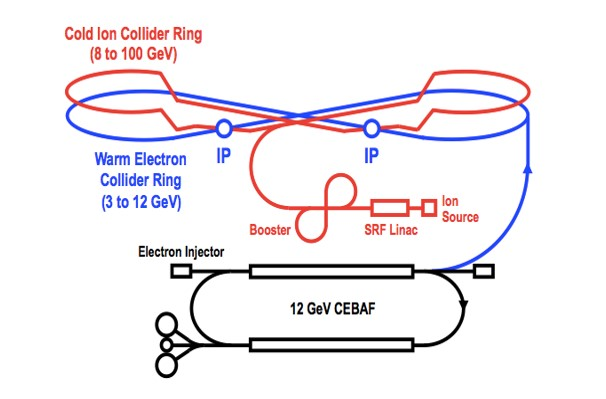
\includegraphics[width=.75\textwidth]{../../img/jleic_schematic.jpg}
	\caption{Schematic of the Jefferson Lab EIC}
	\label{fig:jleic1}
\end{figure}

Table \ref{table:parameters} summarizes some of the relevant design parameters for the machine.  The JLEIC machine is unique, and thus background rates and mitigation choices will be specific to the machine design.  While much can be learned from previous machine experiences, the JLEIC configuration will be the first of its kind and thorough background studies with its specific parameters must be completed.

\begin{center}
	\begin{tabular}{ l l c c c c } 
		JLEIC Parameters & & \multicolumn{2}{c}{Single-turn ERL Cooler} & \multicolumn{2}{c}{Multi-turn ERL Cooler}\\ 
		& & \multicolumn{2}{c}{PEP-II e-ring} & \multicolumn{2}{c}{New e-ring} \\
		\hline \hline
		& & p & e & p & e\\
		\hline
		Beam energy & GeV & 100 & 5 &100 &5 \\ 
		Collision frequency & MHz& \multicolumn{2}{c}{476} & \multicolumn{2}{c}{476}\\ 
		Particles per bunch & $10^10$ & 0.66 & 3.9& 0.98 & 3.7\\
		Beam current & A & 0.5 & 3 & 0.75 & 2.82\\
		Polarization &  & \textgreater80\% & \textgreater80\% & \textgreater80\% & \textgreater80\%\\
		Bunch length, rms & cm & 1 & 1.2 & 1.2 & 1.2 \\
		Norm. emittance, x/y& $\mu$m & 1/0.5 & 144/72 & 0.5/0.1 & 70/14 \\
		x/y $\beta^*$ & cm &4/2 & 2.6/1.3 & 6/1.2 & 4/0.8\\
		Vert. beam-beam param.& & 0.006 & 0.014 & 0.015 & 0.053\\
		Laslett tune shift & & 0.01 & Small & 0.048 & Small\\
		Detector space, up/down & m & 3.6/7 & 2.4/1.6 & 3.6/7 & 2.4/1.6\\
		Hourglass (HG)reduction & & \multicolumn{2}{c}{0.88} & \multicolumn{2}{c}{0.80}\\
		Lumi./IP, w/ HG, $\mathbf{10^{33}}$ & cm$^{-2}$ s$^{-1}$ & \multicolumn{2}{c}{4.6} & \multicolumn{2}{c}{19.5} \\
		\hline
		%\caption{Parameters and luminosity for a full-acceptance detector.}
		\label{table:parameters}
	\end{tabular}
\end{center}

\subsubsection{Interaction Point}

\begin{enumerate}	
\item{\textbf{Detector}}
% how to properly bold enumerate?

The full-acceptance detector region has been placed far from the electron arc exit ($\approx$ 70 m) to minimize the synchrotron radiation background, and close to the ion arc exit to minimize the hadronic background from ion beam scattering on residual gas.  While long, straight section of machine lattice minimizes the synchrotron radiation from magnet bending, it is possible that electron beam scattering on beamline gas interactions could generate enough synchrotron radiation to negatively impact the detectors.  A small upstream chicane has been proposed to mitigate this effect. The quantity and distribution of synchrotron radiation from beam-gas interaction must be evaluated, along with the effectiveness of a chicane.  Such a study is within the scope of this proposal.  
\begin{figure}
	\centering
	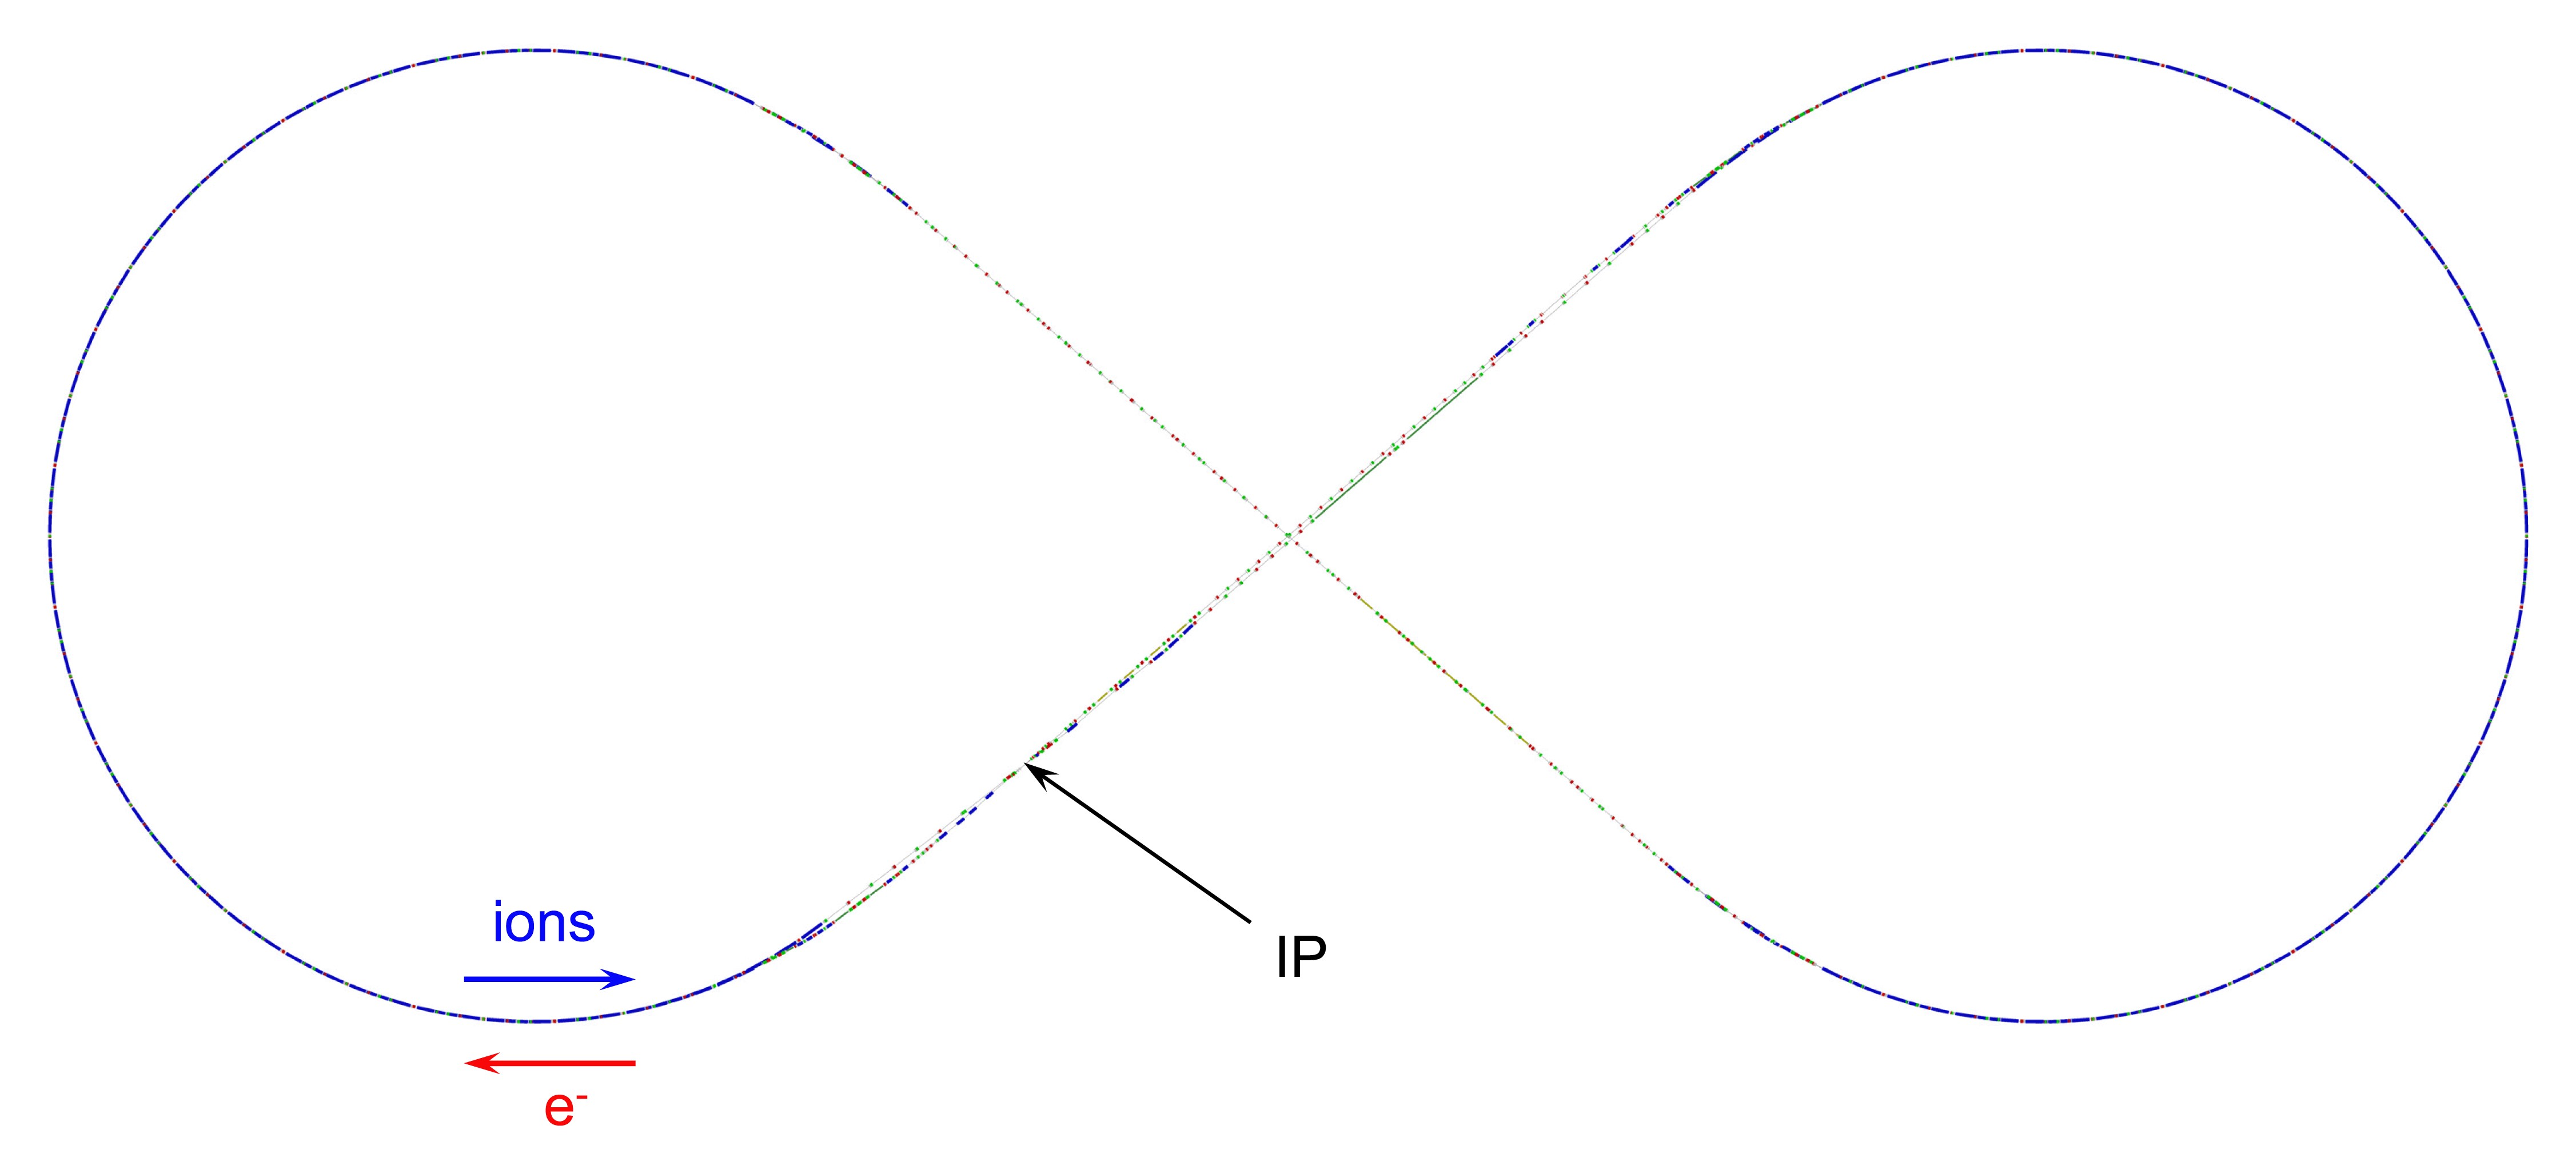
\includegraphics[width=.75\textwidth]{../../img/collider_rings_layout.jpg}
	\caption{Collider rings' Layout.}
	\label{fig:jleic2}
\end{figure}
%edit image with curly brackets to indicate electron and ion beam components also chican Mike mentioned possibly putting in?
\begin{figure}[h!]
	\centering
	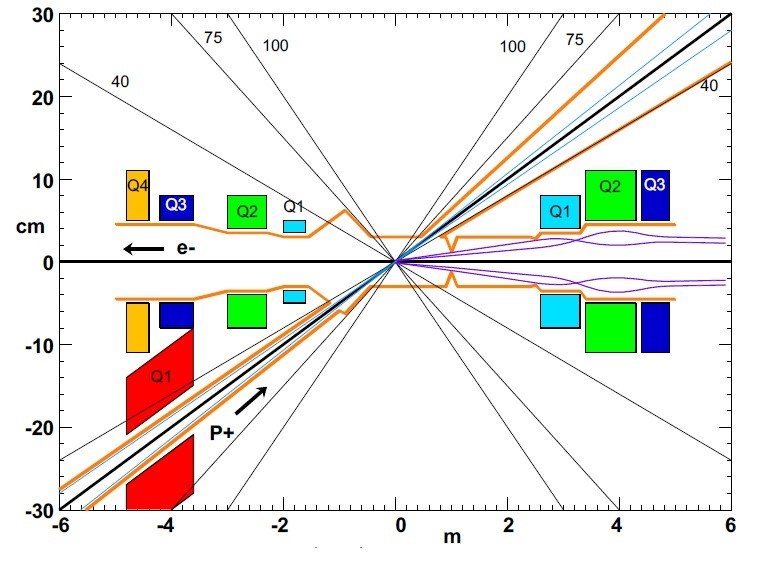
\includegraphics[width=.75\textwidth]{../../img/new_beam_pipe.jpg}
	\caption{Schematic of the JLEIC interaction region beam pipe design.}
	\label{fig:jleic3}
\end{figure}

\begin{figure}[t]
	\centering
	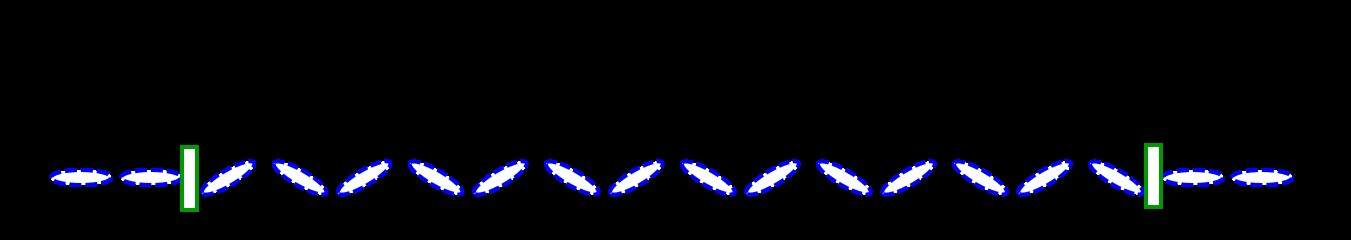
\includegraphics[width=.75\textwidth]{../../img/crab_bunch_profile.jpg}
	\caption{Evolution of the horizontal bunch profile between the crab cavities.}
	\label{fig:jleic4}
\end{figure}

\textbf{\item{Beam Pipe}}

The JLEIC beam pipe concept incorporates several features to minimize background and interaction with beampipe material.  Since the x/y electron beam ratio of 5:1 is quite low, the final focus magnets are stronger for a given electron beam energy than in previous machines.  Thus, it is likely that high power synchrotron radiation will be generated in these quadrupoles and create background in the detector.  The current beam pipe design utiliizes a 50 mrad crossing angle for quick beam separation, and implements masking within the electron pipe to collimate synchrotron radiation, as well as gold coatings to reduce background in the detector.  This study proposes to develop the code needed to implement the beam pipe design in the simulation tools such as GEMC and Molflow+, study the impact of design choices on the quantities of background delivered to the detector, and apply results to improved iterations of this vacuum chamber. 

The beam pipe within the central detector is heavily instrumented and provides minimal access for vacuum pumping ports.  In order to achieve reasonable background rates, the vacuum in the interaction region should be no greater than $10^-9$ mbar during operation.  The vacuum hardware has not been designed yet and collaboration between the accelerator, physics, and vacuum teams are required to produce a robust design for the beam pipe at the IP.

While the beam crossing angle is specific to the JLEIC machine, the beam pipe design and background mitigation choices is of generic interest to both Jefferson and Brookhaven designs.
%insert images of newest beampipe design


\textbf{\item{Crab Crossing}}

The 50 mrad crossing angle provides quick beam separation, minimizing unwanted beam-beam interactions and subsequent background.  The JLEIC design incorporates a local compensation scheme using SRF crab cavities to restore head-on collisions and compensate for the luminosity loss due to the nonzero crossing angle.  

This bunch tilt in the horizontal plane may create hadronic and leptonic background fluctuations which need to be considered.  Both Jefferson and Brookhaven designs incorporate crab cavities, and a quantitative understanding of the background fluctuations is of mutual benefit. 

\end{enumerate}

\subsubsection{Compton Polarimeter}
%\input{../overview/polarimeter.tex}






